\documentclass[t]{beamer}
\usepackage[utf8]{inputenc} % to be able to type unicode text directly
\usepackage{inconsolata} % for a nicer (e.g. non-courier) tt family font

\usepackage{graphicx} % to include figures
\usepackage{hyperref,url} % to make clickable hyperlinks
%\usepackage{minted} % for code insets
%\usepackage{array} %
%\usepackage{bbm} % for blackboard 1

\usepackage{tikz}

\usepackage{soul}
\usepackage{cancel}
\renewcommand{\CancelColor}{\color{red}}

\colorlet{darkgreen}{black!50!green}
\colorlet{ddarkgreen}{black!75!green}
\colorlet{darkred}{black!50!red}
\definecolor{ipol}{rgb}{.36,.29,.65}
\usecolortheme[named=ipol]{structure}
\definecolor{term}{rgb}{.9,.9,.9}

\newcommand{\reference}[1] {{\scriptsize \color{gray}  #1 }}
\newcommand{\referencep}[1] {{\tiny \color{gray}  #1 }}
\newcommand{\unit}[1] {{\tiny \color{gray}  #1 }}

\def\R{\mathbf{R}}
\def\F{\mathcal{F}}
\def\x{\mathbf{x}}
\def\u{\mathbf{u}}
\def\FFT{\mathtt{FFT}}
\def\IFFT{\mathtt{IFFT}}
\DeclareMathOperator*{\argmin}{arg\,min}
\DeclareMathOperator*{\patch}{patch}

% disable spacing around verbatim
\usepackage{etoolbox}
\makeatletter
\preto{\@verbatim}{\topsep=0pt \partopsep=0pt }
\makeatother

\mode<presentation>
\setbeamercolor*{author in head/foot}{parent=none}
\setbeamercolor*{title in head/foot}{parent=none}
\setbeamercolor*{date in head/foot}{parent=none}
\defbeamertemplate*{footline}{infoline theme}
{
  \leavevmode%
  \hfill\color{darkgreen}
   \insertframenumber{} / \inserttotalframenumber\hspace*{2ex}
  \vskip0pt%
}

\makeatletter
\newcommand\SoulColor{%
  \let\set@color\beamerorig@set@color
  \let\reset@color\beamerorig@reset@color}
\makeatother
\newcommand<>{\St}[1]{\only#2{\SoulColor\st{#1}}}
\setstcolor{red}

\mode<all>
\setbeamertemplate{navigation symbols}{}

%\setbeamersize{text margin left=1em,text margin right=1em} (does not work)
%\setbeamersize{text margin left=1em}


\begin{document}

\begin{frame}[plain]
	\vfill
	\vfill
	\begin{center}
		\Large\bf Realtime detection of REVEAL labels
	\end{center}
	\vfill
	\vfill
	Meeting CMLA/SURYS\\
	17--11--2016
\end{frame}

\begin{frame}
	\frametitle{Plan}

	\begin{enumerate}
		\item The CMLA pipeline thus far:
			\begin{enumerate}
				\item Realtime blurred frame detection (mauricio)
				\item Gaussian filtering---no optimization yet
				\item Realtime dark blob detection
				\item Realtime alignment detection
			\end{enumerate}
		\item Thinks we are looking at
			\begin{enumerate}
				\item Constellation matching
				\item 1D techniques
			\end{enumerate}
	\end{enumerate}
\end{frame}

\begin{frame}
	\frametitle{Realtime blurred frame detection (mauricio)}
	{\bf Input:} gray-scale image\\
	{\bf Output:} binary decision whether the image is sharp or blurred

	\bigskip

	Algorithm: check whether the image is contrasted enough and there are
	enough points with high enough gradient.

	\vfill

	%Parameters:\\
	\begin{tabular}{l|l|l}
		parameter & meaning & default value \\
		\hline
		$\Delta_{\mathrm{min}}$ & minimal contrast & 100 gray levels \\
		$g_{\mathrm{th}}$ & minimal gradient & $40.0$ gray/pix \\
		$C_{\mathrm{th}}$ & required nr. of pixels with high gradient & $3000$ \\
		$s_{\mathrm{sat}}$ & saturation threshold & $200$ gray levels \\
		$S_{\mathrm{th}}$ & allowed percent of saturated pixels & $20\%$ \\
	\end{tabular}
\end{frame}

\begin{frame}
	\frametitle{Realtime dark blob detection}
	{\bf Input:} gray-scale image\\
	{\bf Output:} list of points

	\bigskip

	Algorithm: find {\bf local minima} of the $\sigma$-blurred image
	that satisfy two local ``roundness'' criteria.

	\[
		u_{xx}+u_{yy} > \tau
		\qquad
		\qquad
		\qquad
		\frac{u_{xx}u_{yy}-u_{xy}^2}{(u_{xx}+u_{yy})^2}>\kappa
	\]

	\vfill

	%Parameters:\\
	\begin{tabular}{l|l|l}
		parameter & meaning & default value \\
		\hline
		$\sigma$ & size of the pre-filtering & $1.0$ pixels \\
		$\tau$ & strength of the local minimum & $20$ gray/pixel$^2$\\
		$\kappa$ & roundness measure & $0.04$ \\
	\end{tabular}
\end{frame}

\begin{frame}
	\frametitle{Realtime alignment detection}
	{\bf Input:} list of points\\
	{\bf Output:} list of straight lines

	\bigskip

	Algorithm (RANSAC): test many lines determined by several random pairs of
	points and keep the best one.

	\bigskip

	Once an alignment is found, these points are removed from the list and
	RANSAC is run again.

	\vfill

	%Parameters:\\
	\begin{tabular}{l|l|l}
		parameter & meaning & default value \\
		\hline
		$N_{runs}$ & number of times RANSAC is run & $10$ \\
		$N_{trials}$ & number of trials for each RANSAC & $1000$ \\
		$M_{inliers}$ & minimum required number of inliers & $6$ \\
		$\delta$ & distance tolerance & $1.0$ pixels \\
	\end{tabular}
\end{frame}

\begin{frame}
	\frametitle{Summary of performances}

	\begin{enumerate}
		\item Blurred frame detection: no performance penalty ($>30Hz$)
		\item Blob detection: slow, due to  Gaussian pre-filtering (20Hz)
		\item Alignement detection: no performance penalty of $10\times 500$ trials for up to $200$ points ($>30Hz$).
	\end{enumerate}

	\vfill
	Possible optimizations
	\begin{enumerate}
		\item Use a faster, less precise, Gaussian filtering
		\item Detect the points in a multiscale pyramid, to allow smaller~$\sigma$ with equivalent effect.
	\end{enumerate}

\end{frame}

\begin{frame}
	\frametitle{Constellation matching}
	\framesubtitle{What to do if you are lost in space?  This is a solved problem}

	\vfill

	{\scriptsize
	Salomon, P. M., Goss, W. C. \emph{A microprocessor-controlled CCD star tracker.} AIAA, Aerospace Sciences Meeting. {\bf 1976}.

	\bigskip

	Junkins, J. L., White, C.C., Turner, J.D. \emph{Star pattern recognition for real time attitude determination.} Journal of the Astronautical Sciences, {\bf 1977}

	\bigskip

	Liebe, C. C. \emph{Pattern recognition of star constellations for spacecraft applications}. IEEE Aerospace and Electronic Systems Magazine, {\bf 1992}.

	\bigskip

	Spratling, B. B., Mortari, D. \emph{A Survey on Star Identification Algorithms}. Algorithms, {\bf 2009}

	}

	\vfill
	\vfill

	In astronomy, constellation matching is easier, because only three
	parameters need to be found (the orientation of the camera).  Detecting
	REVEAL labels is harder because there are more parameters (projection,
	label deformation).
\end{frame}

\begin{frame}
	\frametitle{1D techniques}
	\framesubtitle{QR codes are trivial to detect in realtime.  Why?}

	\begin{tabular}{cc}
		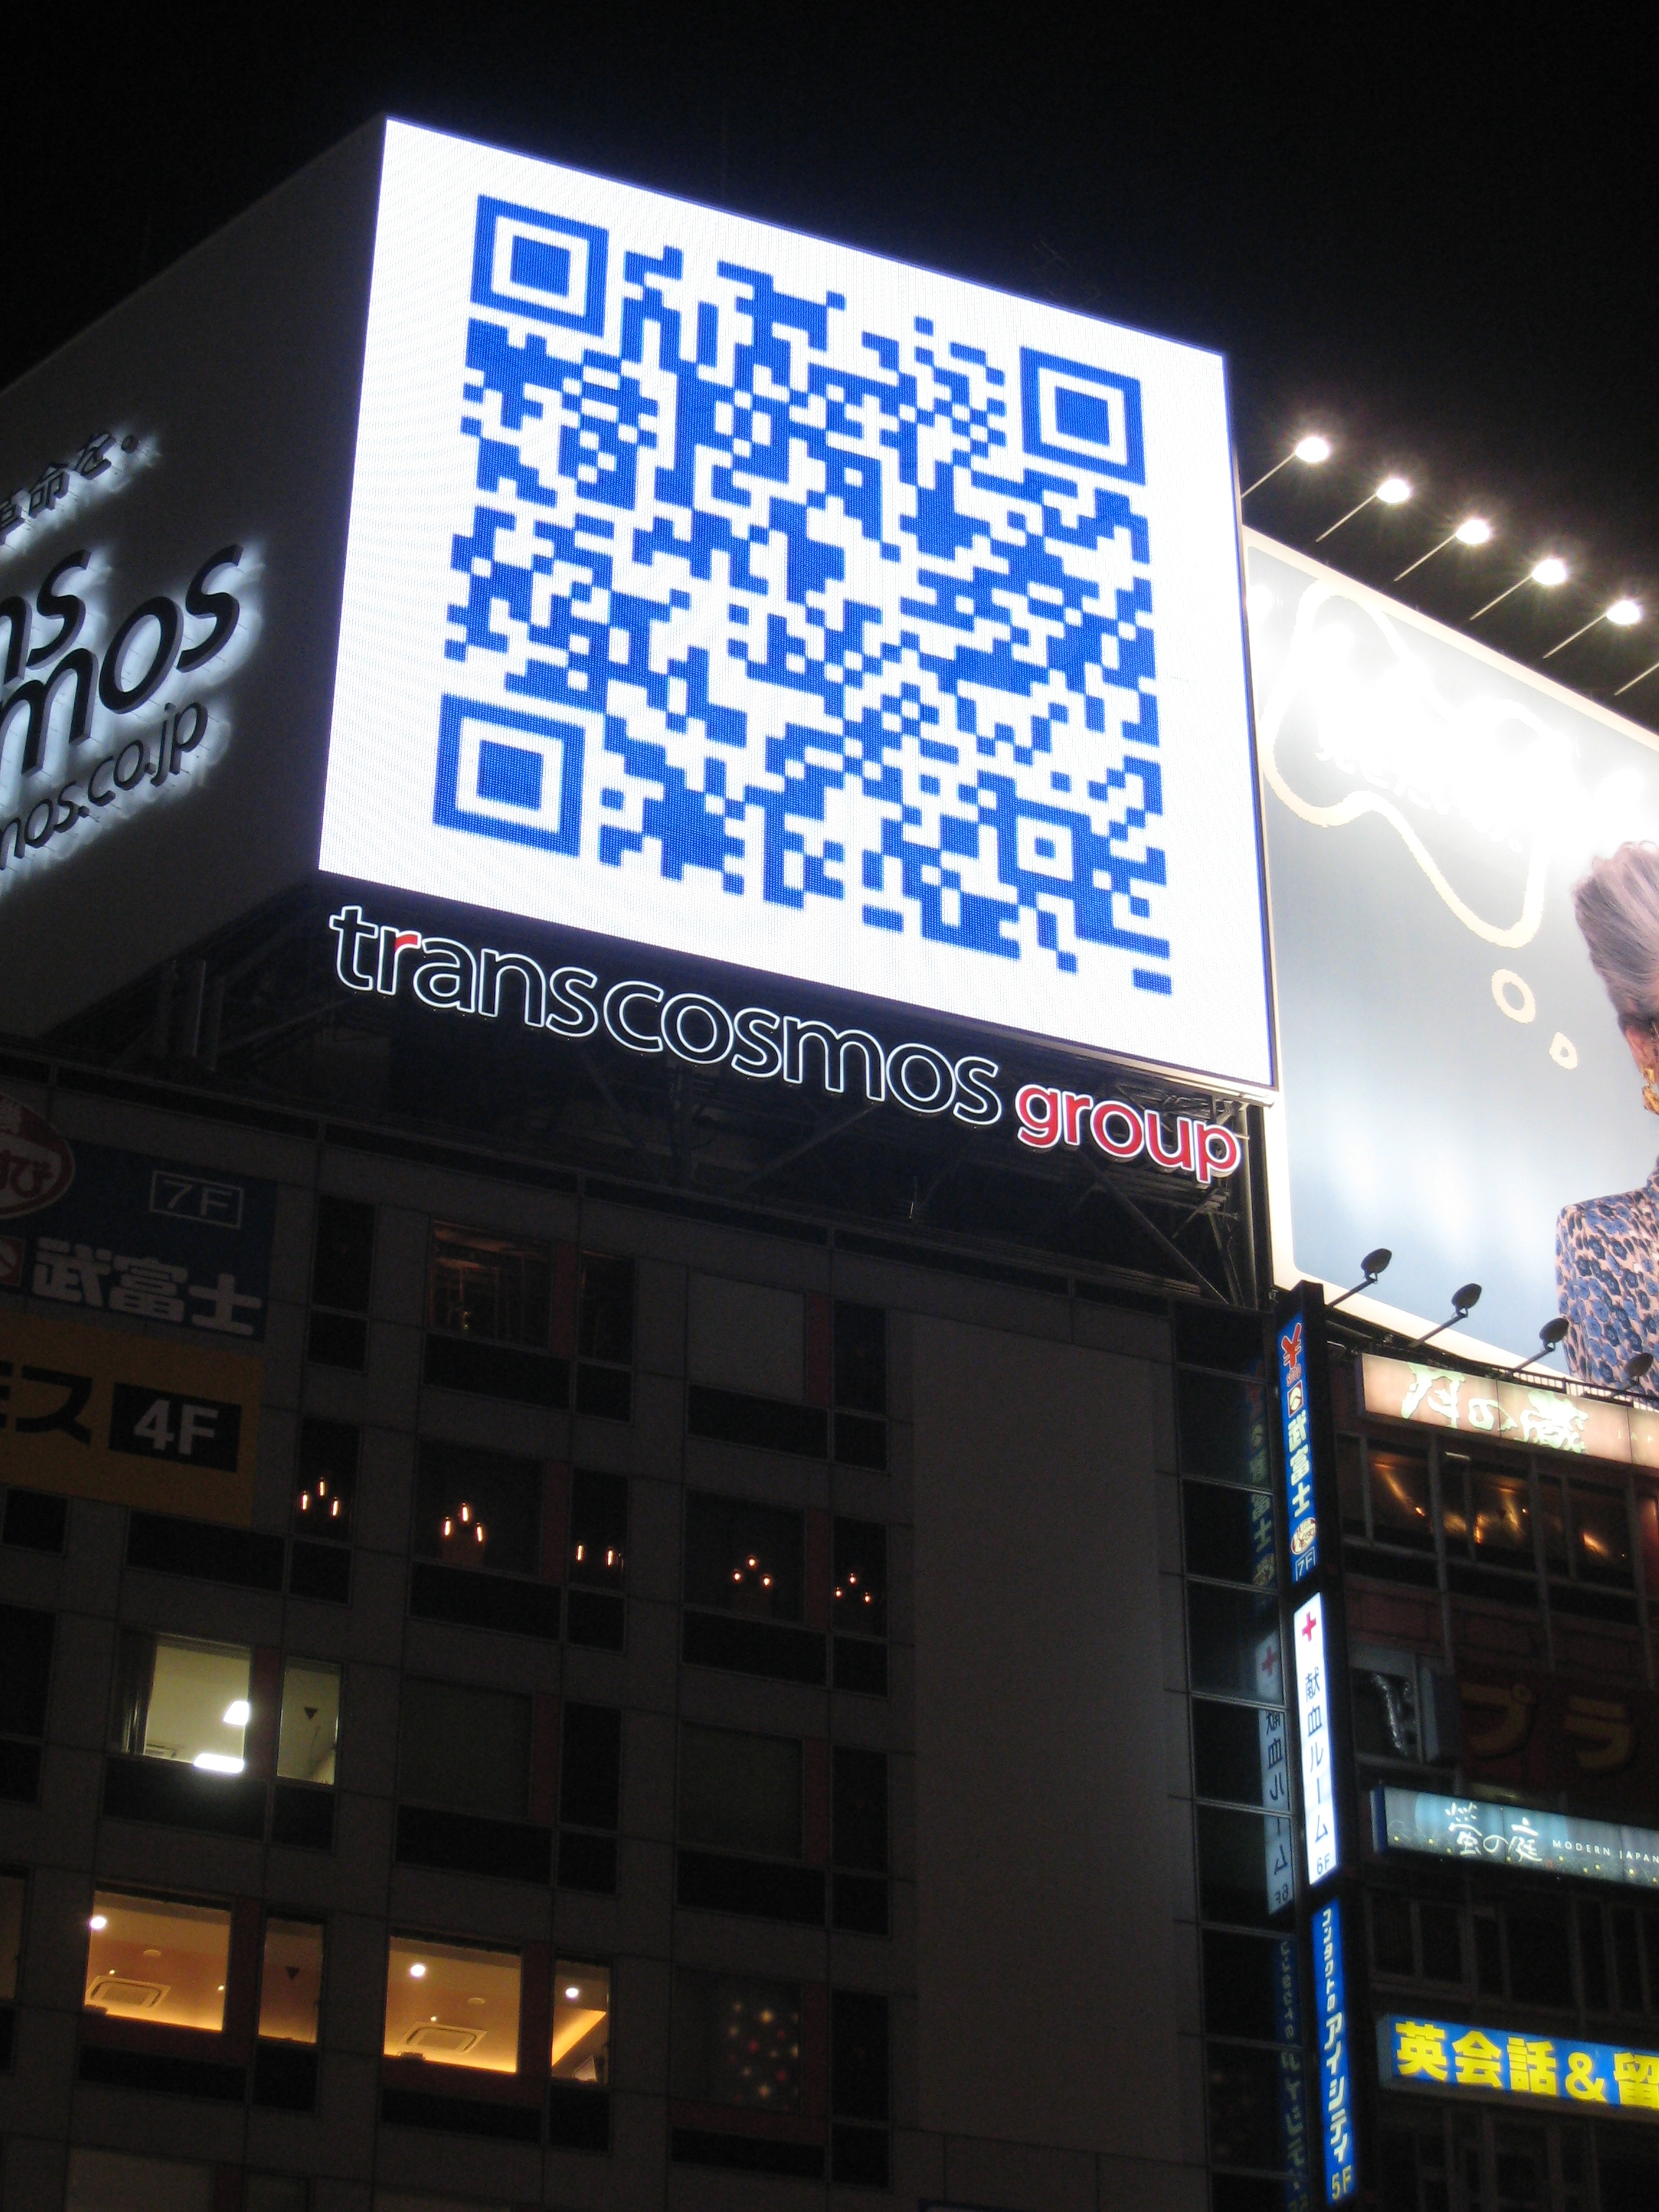
\includegraphics[width=0.45\linewidth]{f/qrbillboard.jpg}&
		\pause
		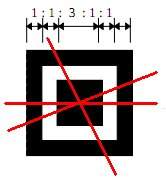
\includegraphics[width=0.45\linewidth]{f/qrpattern.jpg}\\
	\end{tabular}

	Because the 3 corners can be detected by scanning 1D lines.

\end{frame}

\begin{frame}
	\vfill
	demo: pipeline parameters visualization

\end{frame}

\end{document}


% vim:sw=4 ts=4 spell spelllang=en:
